\documentclass{article}
\usepackage[utf8]{inputenc}
\usepackage{graphicx}
\usepackage{amsmath}

\title{Computer graphics - Cylinder and its Normal}
\author{Chassot Samuel, Chraibi Ghali and Nunes Silva Daniel Filipe}
\date{February 2019}

\usepackage{natbib}
\usepackage{graphicx}

\begin{document}

\maketitle

\section{Infinite length cylinder}
Let us take a cylinder with axis vector $c + \textit{k} v_a$ and radius $\textit{r}$. A point $q = (x,y,z)$ is on the cylinder iif the its distance from the axis vector $c + \textit{k} v_a$ (length of the red line $l$ on the Figure 1) is equal to $\textit{r}$.

\begin{figure}[h]
\centering
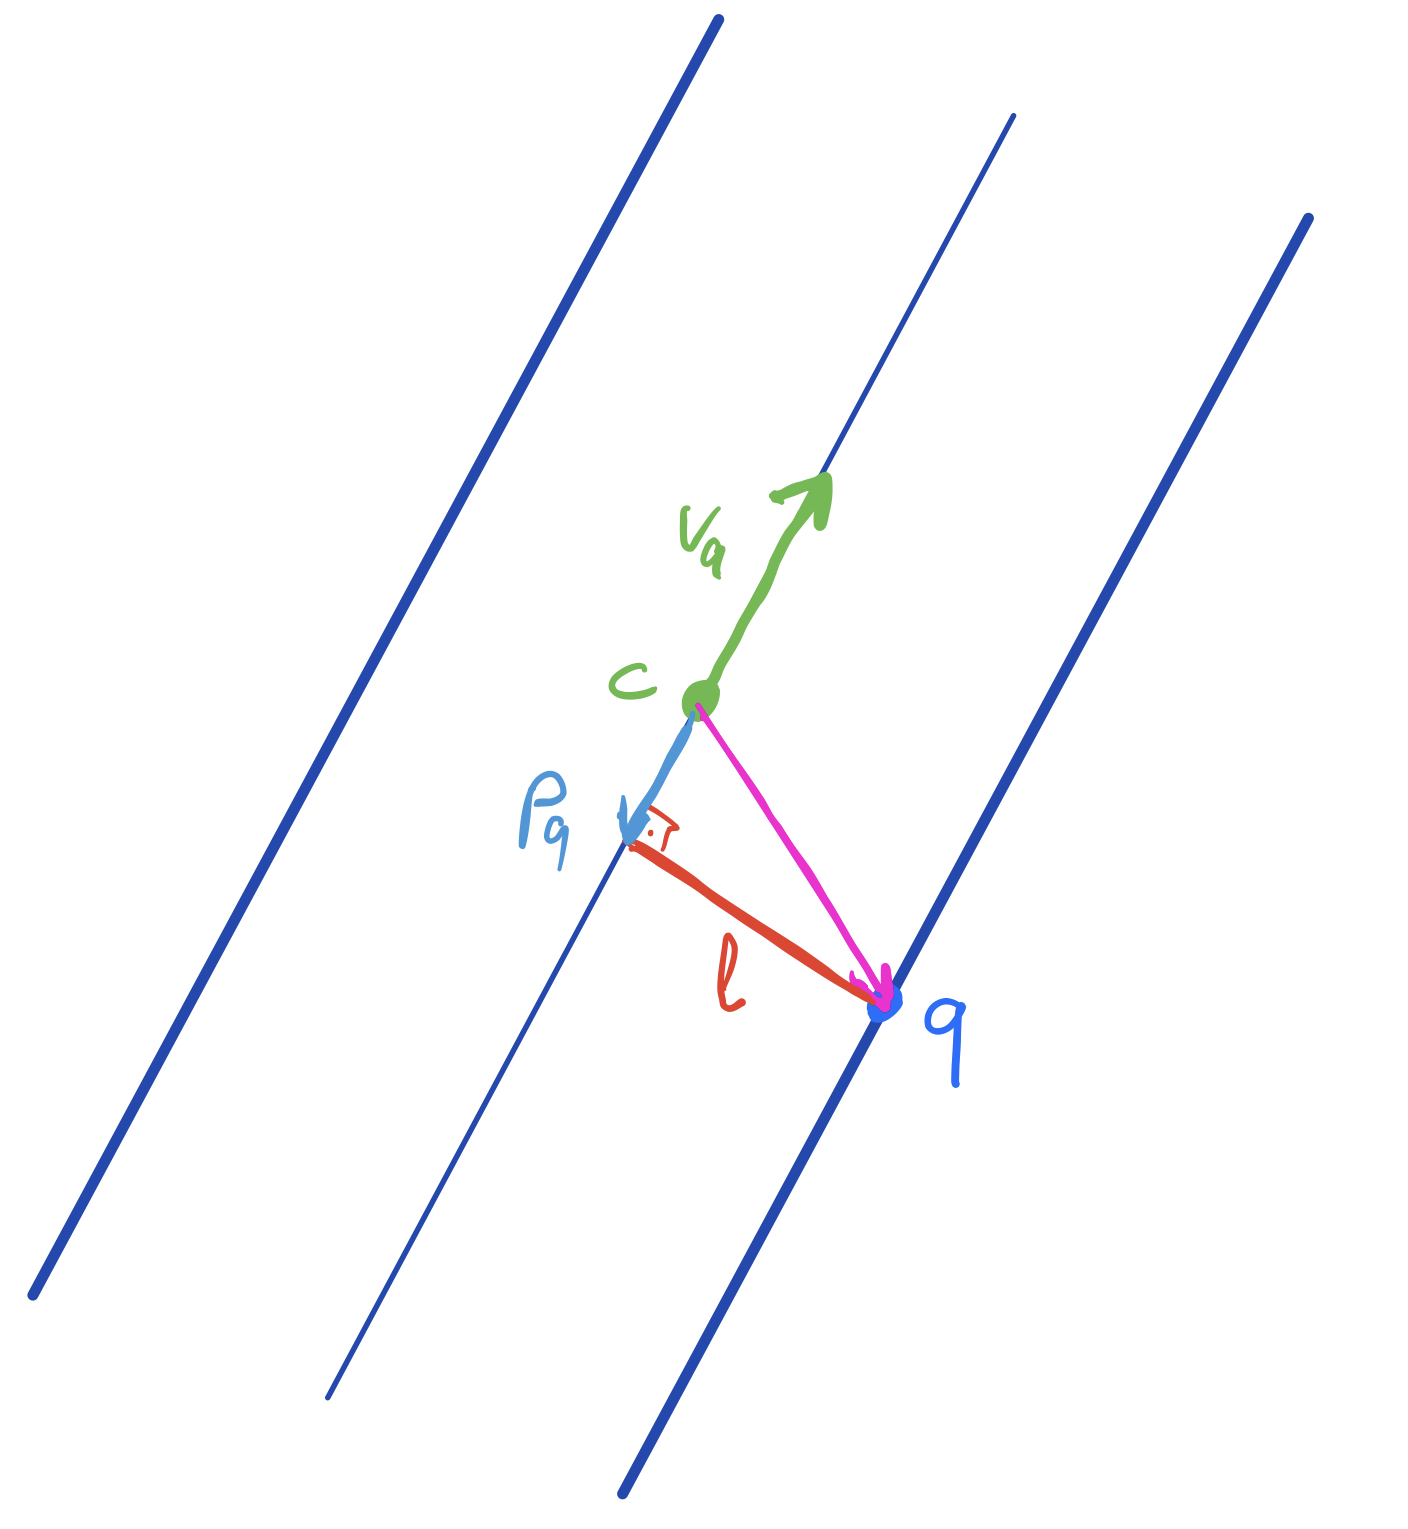
\includegraphics[width=6cm]{res/Cylinder_sketch.jpeg}
\caption{Cylinder}
\end{figure}

First, we need to compute the orthogonal projection $p_q$ of the vector $\overrightarrow{cq}$ on $v_a$ :
$$p_q = \langle v_a, q-c\rangle  v_a$$

Then, we can compute the vector $l$ :
\begin{align*}
    &l = q-c-p_q \\
    &l = q-c - \langle v_a, q-c\rangle  v_a
\end{align*}

Finally, we compute the norm of $l$ to get the distance we wanted. We can take this distance squared to simplify computation and we get the following implicit equation for the cylinder:
\begin{gather*}
    |q-c-\langle v_a, q-c\rangle  v_a|^2 - r^2 = 0
\end{gather*}

Now, we inject the ray parametrization of point $q$ :
\begin{gather*}
    q=p+tv \\
    |p-c+tv-\langle v_a, p-c+tv\rangle v_a|^2-r^2=0
\end{gather*}

And solve this equation for $t$ :
\begin{gather*}
    |p-c+tv-\langle v_a, p-c+tv\rangle v_a|^2-r^2=0\\
    |p-c+tv - \langle v_a, p-c\rangle v_a - t\langle v_a, v\rangle v_a|^2 -r^2=0\\
    |t(v+\langle v_a, v\rangle v_a) + (p-c- \langle v_a, p-c\rangle v_a)|^2 -r^2 = 0
\end{gather*}

Let us define the following vectors :
\begin{gather*}
    e = (v-\langle v_a, v\rangle v_a)\\
    f = (p-c- \langle v_a, p-c\rangle v_a)
\end{gather*}

Then :
\begin{gather*}
    |te + f|^2 -r^2 = 0\\
    \langle te+f, te+f\rangle  -r^2 = 0\\
    t^2  \langle e,e\rangle  + t\langle e+f, e+f\rangle  + \langle f,f\rangle  -r^2 = 0
\end{gather*}

We end up with an equation of the form:
$$t^2A + tB + C = 0$$

Where :
\begin{align*}
    A &= \langle e,e\rangle  \\
    &= |v-\langle v_a, v\rangle v_a|^2\\
    B &= 2\langle e, f\rangle  \\
    &= 2\langle v-\langle v_a, v\rangle v_a, p-c- \langle v_a, p-c\rangle v_a\rangle \\
    C &= \langle f,f\rangle  -r^2 \\
    &= |p-c- \langle v_a, p-c\rangle v_a|^2
\end{align*}


Now, we can resolve the previous equation for $t$ using \textit{quadraticSolve} and store the solution(s) in $S$.

\section{Finite length cylinder}
The array $S$ may contain zero, one or two solutions. Valid solutions must be positive and if there are two valid solutions for $s$, we should keep the smalllest one, which is inside the defined cylinder (radius $r$ and height $h$).

First, we remove negative values from $S$. Then, we keep the $t_i$'s such that $p_i = p+t_iv$ are on the finite length cylinder.

To do so, we compute the orthogonal projection of the vector between $c$ and the intersection point $p_i$ on $v_a$ and check if its norm is smaller than $h/2$ :
$$|\langle p_i-c, v_a\rangle v_a|^2 \leq h/2$$
And keep the smallest $t_i$ satisfying this inequation.

\section{Normal to cylinder surface}

The normal to the cylinder surface at point $p_i$ is computed as the vector from the orthogonal projection $proj_{p_i}$ of $p_i$ on $v_a$ to $p_i$.

\begin{figure}[h]
\centering
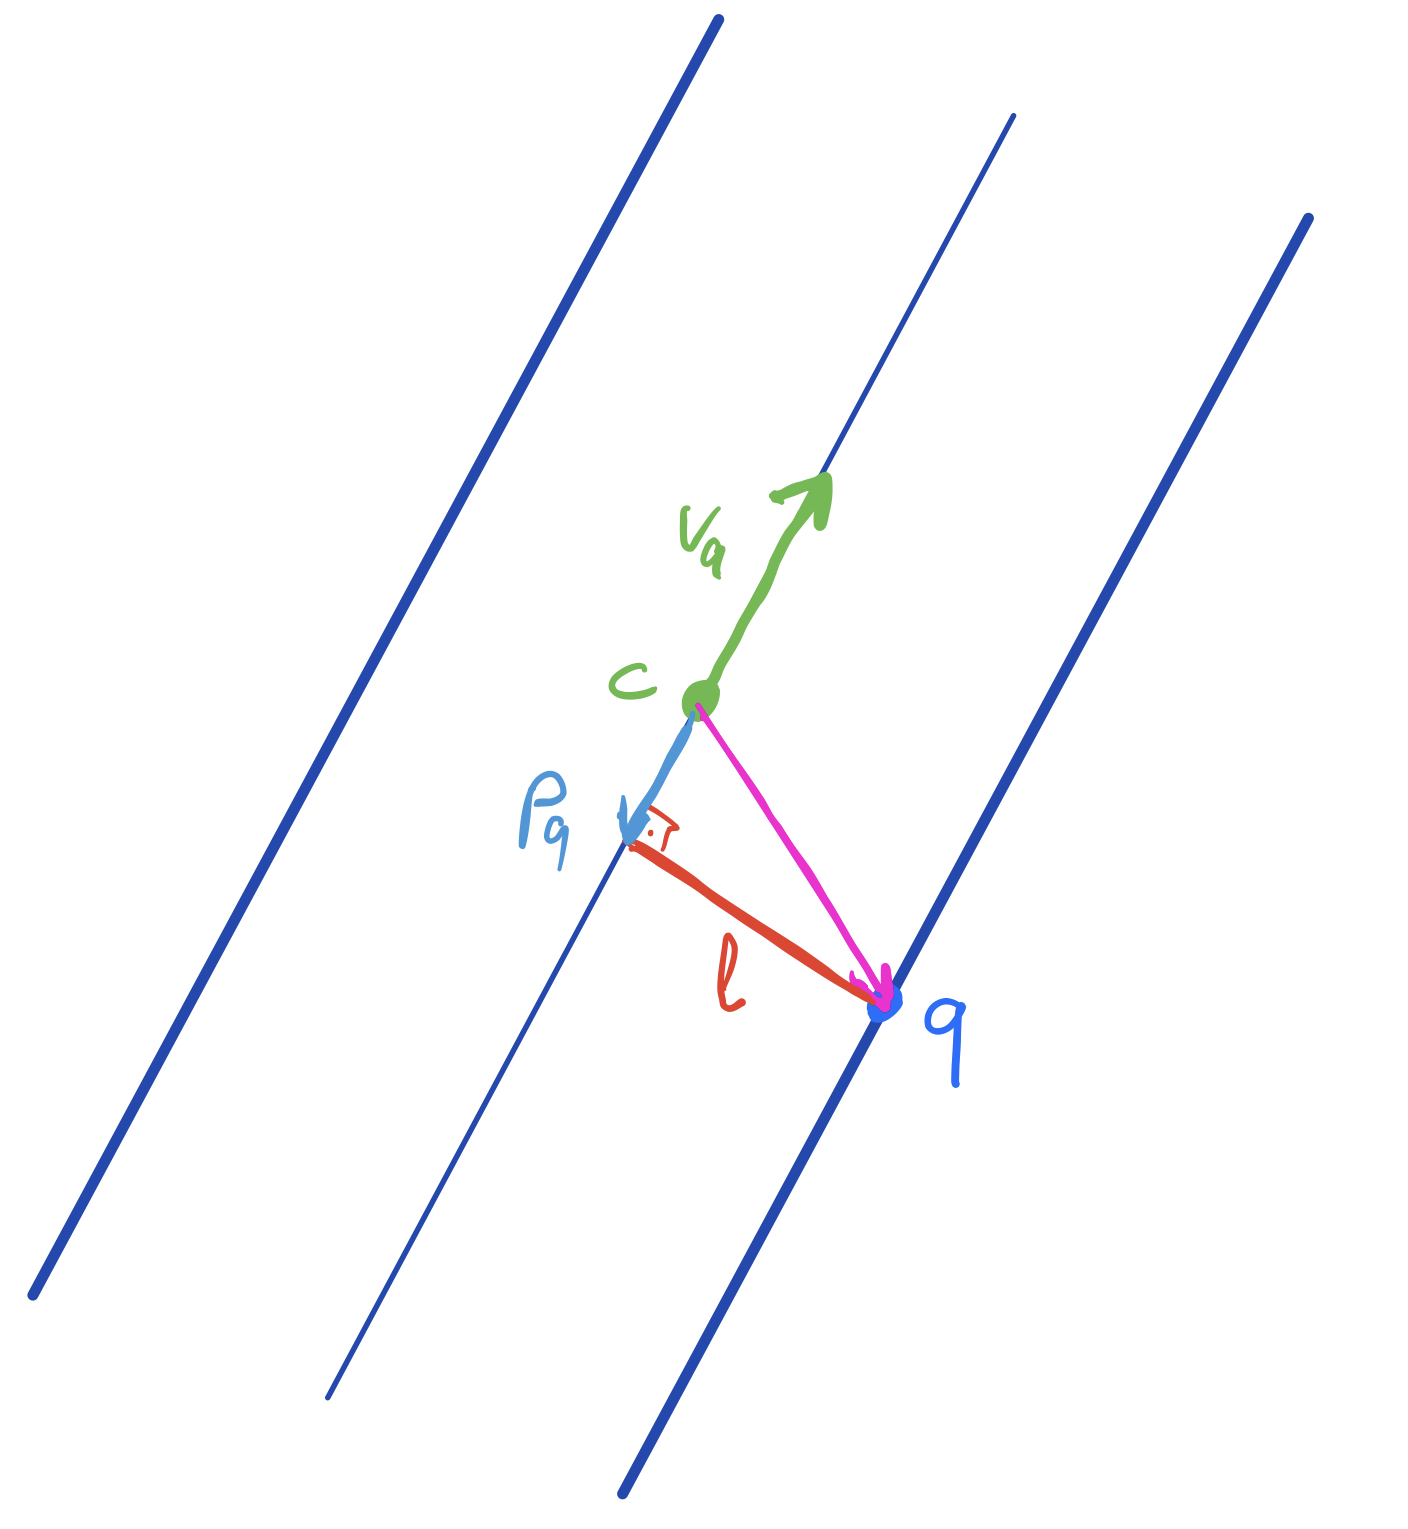
\includegraphics[width=6cm]{res/Cylinder_sketch.jpeg}
\caption{Normal}
\end{figure}


\begin{align*}
    &proj_{p_i} = c + \langle p_i-c, v_a \rangle \\
    &n = p_i - proj_{p_i}
\end{align*}

As there are two possible directions for the vector $v$, we choose the one \textit{pointing againt the ray direction}. In other words, the dot product of $v$ and $n$ must be negative. Otherwise, we have to take the inverse $n$ by multiplying its components by $-1$.

\end{document}
